% Options for packages loaded elsewhere
\PassOptionsToPackage{unicode}{hyperref}
\PassOptionsToPackage{hyphens}{url}
\PassOptionsToPackage{dvipsnames,svgnames,x11names}{xcolor}
%
\documentclass[
  12pt,
]{article}
\usepackage{amsmath,amssymb}
\usepackage{lmodern}
\usepackage{setspace}
\usepackage{iftex}
\ifPDFTeX
  \usepackage[T1]{fontenc}
  \usepackage[utf8]{inputenc}
  \usepackage{textcomp} % provide euro and other symbols
\else % if luatex or xetex
  \usepackage{unicode-math}
  \defaultfontfeatures{Scale=MatchLowercase}
  \defaultfontfeatures[\rmfamily]{Ligatures=TeX,Scale=1}
\fi
% Use upquote if available, for straight quotes in verbatim environments
\IfFileExists{upquote.sty}{\usepackage{upquote}}{}
\IfFileExists{microtype.sty}{% use microtype if available
  \usepackage[]{microtype}
  \UseMicrotypeSet[protrusion]{basicmath} % disable protrusion for tt fonts
}{}
\makeatletter
\@ifundefined{KOMAClassName}{% if non-KOMA class
  \IfFileExists{parskip.sty}{%
    \usepackage{parskip}
  }{% else
    \setlength{\parindent}{0pt}
    \setlength{\parskip}{6pt plus 2pt minus 1pt}}
}{% if KOMA class
  \KOMAoptions{parskip=half}}
\makeatother
\usepackage{xcolor}
\usepackage[left=2.5cm,right=2.5cm,top=2cm,bottom=2cm]{geometry}
\usepackage{longtable,booktabs,array}
\usepackage{calc} % for calculating minipage widths
% Correct order of tables after \paragraph or \subparagraph
\usepackage{etoolbox}
\makeatletter
\patchcmd\longtable{\par}{\if@noskipsec\mbox{}\fi\par}{}{}
\makeatother
% Allow footnotes in longtable head/foot
\IfFileExists{footnotehyper.sty}{\usepackage{footnotehyper}}{\usepackage{footnote}}
\makesavenoteenv{longtable}
\usepackage{graphicx}
\makeatletter
\def\maxwidth{\ifdim\Gin@nat@width>\linewidth\linewidth\else\Gin@nat@width\fi}
\def\maxheight{\ifdim\Gin@nat@height>\textheight\textheight\else\Gin@nat@height\fi}
\makeatother
% Scale images if necessary, so that they will not overflow the page
% margins by default, and it is still possible to overwrite the defaults
% using explicit options in \includegraphics[width, height, ...]{}
\setkeys{Gin}{width=\maxwidth,height=\maxheight,keepaspectratio}
% Set default figure placement to htbp
\makeatletter
\def\fps@figure{htbp}
\makeatother
\setlength{\emergencystretch}{3em} % prevent overfull lines
\providecommand{\tightlist}{%
  \setlength{\itemsep}{0pt}\setlength{\parskip}{0pt}}
\setcounter{secnumdepth}{-\maxdimen} % remove section numbering
\newlength{\cslhangindent}
\setlength{\cslhangindent}{1.5em}
\newlength{\csllabelwidth}
\setlength{\csllabelwidth}{3em}
\newlength{\cslentryspacingunit} % times entry-spacing
\setlength{\cslentryspacingunit}{\parskip}
\newenvironment{CSLReferences}[2] % #1 hanging-ident, #2 entry spacing
 {% don't indent paragraphs
  \setlength{\parindent}{0pt}
  % turn on hanging indent if param 1 is 1
  \ifodd #1
  \let\oldpar\par
  \def\par{\hangindent=\cslhangindent\oldpar}
  \fi
  % set entry spacing
  \setlength{\parskip}{#2\cslentryspacingunit}
 }%
 {}
\usepackage{calc}
\newcommand{\CSLBlock}[1]{#1\hfill\break}
\newcommand{\CSLLeftMargin}[1]{\parbox[t]{\csllabelwidth}{#1}}
\newcommand{\CSLRightInline}[1]{\parbox[t]{\linewidth - \csllabelwidth}{#1}\break}
\newcommand{\CSLIndent}[1]{\hspace{\cslhangindent}#1}
\usepackage[labelsep=period]{caption}
\usepackage[labelfont=bf]{caption}
\usepackage{booktabs}
\usepackage{caption}
\usepackage{microtype}
\usepackage{sectsty}
\captionsetup[figure]{font=small}
\captionsetup[table]{font=small}
\captionsetup[table]{justification=justified}
\captionsetup[figure]{justification=justified}
\usepackage[default]{sourcesanspro}
\usepackage{booktabs}
\usepackage{longtable}
\usepackage{array}
\usepackage{multirow}
\usepackage{wrapfig}
\usepackage{float}
\usepackage{colortbl}
\usepackage{pdflscape}
\usepackage{tabu}
\usepackage{threeparttable}
\usepackage{threeparttablex}
\usepackage[normalem]{ulem}
\usepackage{makecell}
\usepackage{xcolor}
\ifLuaTeX
  \usepackage{selnolig}  % disable illegal ligatures
\fi
\IfFileExists{bookmark.sty}{\usepackage{bookmark}}{\usepackage{hyperref}}
\IfFileExists{xurl.sty}{\usepackage{xurl}}{} % add URL line breaks if available
\urlstyle{same} % disable monospaced font for URLs
\hypersetup{
  colorlinks=true,
  linkcolor={teal},
  filecolor={Maroon},
  citecolor={teal},
  urlcolor={teal},
  pdfcreator={LaTeX via pandoc}}

\author{}
\date{\vspace{-2.5em}}

\begin{document}

\captionsetup{justification=raggedright,singlelinecheck=false}
\pagenumbering{gobble}

%\begin{titlepage}
\begin{center}
\vspace*{2\baselineskip}
\Huge
\textbf{TITLE}\\
\vspace*{1\baselineskip}
\Large{by Natasha Louise Hopkins}\\
\vspace*{2\baselineskip}
\Large{\textbf{Master of Biology (Honours), Molecular Cell Biology}}\\
\Large{University of York, UK}\\
\vspace*{2\baselineskip}
\Large{\textbf{Project Director}}\\
Prof. Robert J White\\
\vspace*{2\baselineskip}
\Large{\textbf{Examination Date}}\\
17 April, 2023\\
\vspace*{2\baselineskip}
\Large{\textbf{Word Count}}\\
Abstract: \\
Main: \\
\vspace*{2\baselineskip}
\begin{figure}[h!]
\centering
  
\includegraphics[width=8cm]{../images/uoy_logo.png}
  \label{}
\end{figure}
\end{center}
% \end{titlepage}

%\begin{body}
\hypersetup{linkcolor = black}
\newpage
\tableofcontents
\hypersetup{linkcolor = teal}
\newpage
\setlength{\columnsep}{25pt}
\pagenumbering{arabic}
\linespread{2}
\setlength{\parindent}{0pt}
\huge
\textbf{TITLE}\\
\normalsize
\textbf{Natasha L. Hopkins}\\

\setstretch{1.2}
Abstract

\normalsize
\begin{flushright}
1 Words
\end{flushright}
\hrulefill\\
\setlength{\parindent}{10pt}

\hypertarget{introduction}{%
\section{Introduction}\label{introduction}}

\hypertarget{foxa1-expression-and-erux3b1-breast-cancer}{%
\subsection{FOXA1 Expression and ERα+ Breast Cancer}\label{foxa1-expression-and-erux3b1-breast-cancer}}

\hypertarget{trnas-and-gene-expression}{%
\subsection{tRNAs and Gene Expression}\label{trnas-and-gene-expression}}

\begin{center}\rule{0.5\linewidth}{0.5pt}\end{center}

\hypertarget{materials-methods}{%
\section{Materials \& Methods}\label{materials-methods}}

\hypertarget{acquisition-of-public-chip-seq-datasets}{%
\subsection{Acquisition of Public ChIP-seq Datasets}\label{acquisition-of-public-chip-seq-datasets}}

ChIP-seq was performed on genetically modified MCF7L cells (\emph{insertion, using a lentiviral cDNA delivery system to express Dox-inducible FOXA1})\textsuperscript{{[}\protect\hyperlink{ref-fu2019}{1}{]}}.
Datasets were deposited into the National Centre for Biotechnology Information (NCBI) Sequence Read Archive (SRA)\textsuperscript{{[}\protect\hyperlink{ref-leinonen2010}{2}{]}} under accession no.
PRJNA512997 (Table \ref{tab:data}).
Using ``Genetic Manipulation Tools'' within the Galaxy\textsuperscript{{[}\protect\hyperlink{ref-thegala2022}{3}{]}} environment (v 23.0.rc1), SRAs were converted to FastQ files.
FastQ files were then aligned to the human genome assembly GRCh37 (hg19) using Bowtie2 (v 2.5.0)\textsuperscript{{[}\protect\hyperlink{ref-langmead2012}{4}{]}} to output BAM files.

\begin{longtable}[]{@{}lllll@{}}
\caption{\label{tab:data}Publicly available ChIP-seq SRA files aquired from the NCBI SRA database (accession no. PRJNA512997).}\tabularnewline
\toprule()
Experiment & SRA & Factor & Tissue & Assembly \\
\midrule()
\endfirsthead
\toprule()
Experiment & SRA & Factor & Tissue & Assembly \\
\midrule()
\endhead
PRJNA512997 & SRR8393424 & FOXA1 & MCF-7LP & GRCh37 (Hg19) \\
& SRR8393425 & & & \\
& SRR8393426 & & & \\
& SRR8393427 & H3K27ac & & \\
& SRR8393428 & & & \\
& SRR8393431 & None (input) & & \\
& SRR8393432 & & & \\
\bottomrule()
\end{longtable}

\hypertarget{easeq-for-chip-seq-peak-quantification}{%
\subsubsection{EaSeq for Chip-seq Peak Quantification}\label{easeq-for-chip-seq-peak-quantification}}

BAM files were uploaded into EaSeq (v1.111) as ``Datasets'' using the standard settings for Chip-seq data.
GRCh37 (hg19) tRNA sequences (n = 606) were downloaded as a ``Geneset'' from the UCSC Table Browser\textsuperscript{{[}\protect\hyperlink{ref-Karolchik2004}{5}{]}}, (available at \url{https://genome.ucsc.edu}).
High-confidence tRNAs (n = 416) identified in the GtRNAdb\textsuperscript{{[}\protect\hyperlink{ref-Chan2016}{6}{]}} were extracted as a ``Regionset''.

Signal peak intensities surrounding tRNAs were quantified using the EaSeq ``quantify'' tool.
Here the default settings ``Normalize to reads per million'' and ``Normalize counts to DNA-fragments'' were left checked.
The default setting ``Normalise to a signal of 1000 bp'' was unchecked.
The window size was offset ±500bp from the start of each tRNA gene.
Outputs are referred to as ``Q-values''.

To quantify upstream and downstream signals, the ``quantify'' tool was used with adjusted window sizes.
The upstream region was defined as 500 bp preceding and the first nucleotide of tRNA loci.
Thus, the start position was offset to 0 bp, and the end position was offset to -500 bp.
The downstream region constitutes the 500 bp region beginning with the first nucleotide of tRNA gene body.
The start position was offset to 1 bp, and the end position was offset to 500 bp.

Following quantification, tRNA binding events were arranged in ascending order -DOX Q-value and visualised as heatmaps.
Data was also visualised with ``average'', and ``overlay'' EaSeq tools.

EaSeq\textsuperscript{{[}\protect\hyperlink{ref-lerdrup2016}{7}{]}} is avaiable at \url{http://easeq.net}.

\hypertarget{motif-analysis}{%
\subsection{Motif Analysis}\label{motif-analysis}}

Multiple EM for Motif Elicitation ChIP (MEME) Suite

\hypertarget{statistics}{%
\subsection{Statistics}\label{statistics}}

Statistical tests and graphs were generated with R\textsuperscript{{[}\protect\hyperlink{ref-r}{8}{]}} (v 4.2.3), R Studio\textsuperscript{{[}\protect\hyperlink{ref-rstudio}{9}{]}} (v 2023.03.0.386) and the tidyverse\textsuperscript{{[}\protect\hyperlink{ref-wickham2019}{10}{]}} package.

\begin{center}\rule{0.5\linewidth}{0.5pt}\end{center}

\hypertarget{results}{%
\section{Results}\label{results}}

\hypertarget{binding-of-foxa1-and-h3k27ac-to-trna-genes}{%
\subsection{Binding of FOXA1 and H3k27ac to tRNA Genes}\label{binding-of-foxa1-and-h3k27ac-to-trna-genes}}

To investigate the impact of FOXA1 on tRNA enhancers in ER+ MCF-7 cells, public ChIP-Seq datasets from Fu et al.~(2019)\textsuperscript{{[}\protect\hyperlink{ref-fu2019}{1}{]}} were interrogated.
In this paper, a doxycycline (Dox) inducible OE system was used to achieve FOXA1 OE akin to tamoxifen-resistant (TamR) MCF-7 cells\textsuperscript{{[}\protect\hyperlink{ref-fu2019}{1}{]}}.

FOXA1 and H3K27ac peaks of 416 high-confidence tRNAs were quantified relative to the ±500 bp flanking regions.
Mapped reads of FOXA1 and H3K27ac binding were visualised as heatmaps and ordered by increasing -DOX Q-value.
This revealed a concentration of FOXA1 and H3k27ac at approximately half of tRNAs, relative to ±10 kb flanking regions.
Upon FOXA1 OE, FOXA1 binding increased at a small proportion of tRNAs genes and H3K27ac binding decreases at approximately half of tRNA genes (Figure \ref{fig:results-1}A).
This was confirmed by average signal intensity plots of FOXA1 and H3K27ac binding (Figure \ref{fig:results-1}B).
Input reads generated minimal peak enrichment (Supplementary Figure X).

Peaks were classified as binding events if Q-values exceeded the input values.
FOXA1 interacted with 329 (79.1\%) of tRNA genes, decreasing to 319 (76.7\%) with FOXA1 OE. H3K27ac interacted with 293 (70.4\%) of tRNA genes, decreasing to 266 (63.9\%) with FOXA1 OE (Figure \ref{fig:results-1}C).
Upon FOXA1 OE, mean Q-values significantly increased 1.18-fold for FOXA1 binding (p \textless{} 0.0001), and significantly decreased 0.86-fold for H3K27ac (p \textless{} 0.01) (Supplementary Figures X).
However, FOXA1 OE leads to a significant difference in FOXA1 and H3K27ac binding between individual tDNAs (p \textless0.0001) (Figure \ref{fig:results-1}D).

Together, these results support the notion that FOXA1 overexpression alters the binding landscape of FOXA1 and H3K27ac at tRNAs.

\begin{figure}[H]

{\centering 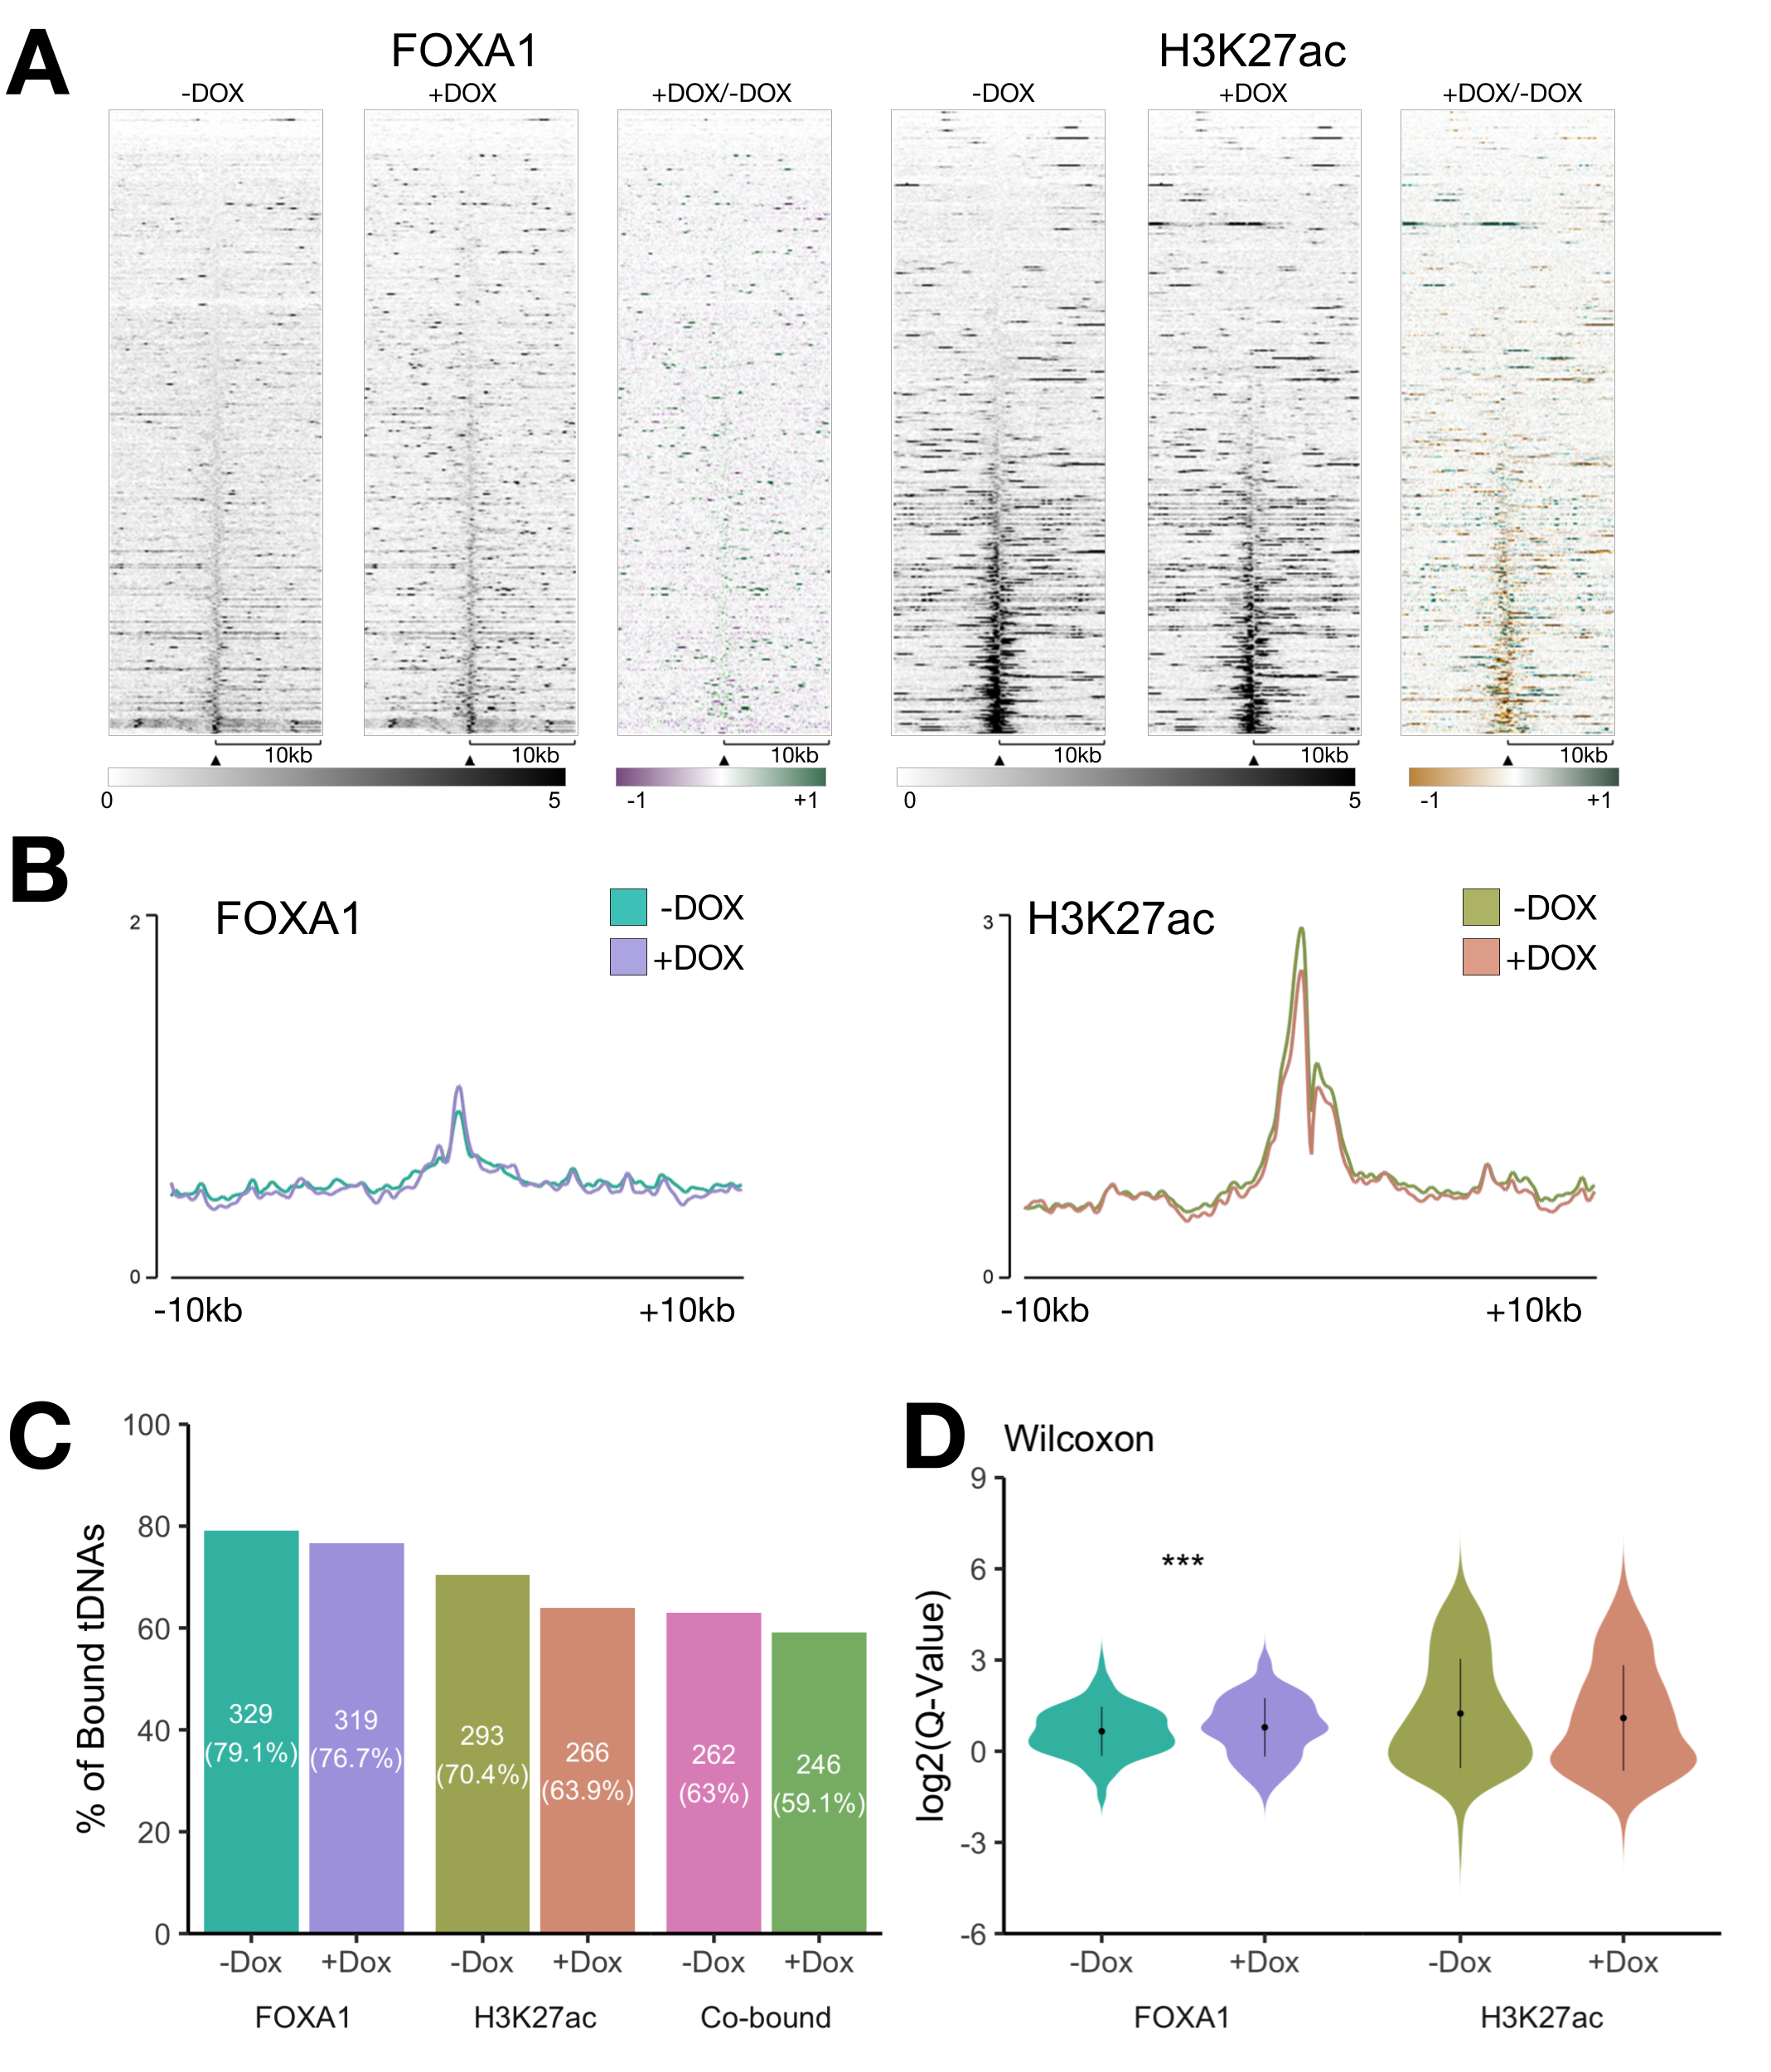
\includegraphics[width=1\linewidth]{../images/results-01} 

}

\caption{(B) Ratiometric heatmaps of the log2 ratio between the binding of FOXA1 or H3k27ac with endogenous FOXA1 expression vs. the binding of FOXA1 or H3k27ac with FOXA1 OE.}\label{fig:results-1}
\end{figure}

\hypertarget{figure-2}{%
\subsection{Figure 2}\label{figure-2}}

\hypertarget{why}{%
\subsubsection{Why}\label{why}}

Using Q-values, tRNAs that are differently enriched upon FOXA1 OE were categorised as `GAIN' or `LOSS'.
This discovered substantially more tRNAs with increased (GAIN) than decreased (LOSS) FOXA1 (92 vs.~21) (Figure \ref{fig:results-2}A).

However, for H3K27ac, the number of tRNAs with an increase (GAIN) was comparable to those with a decrease (LOSS) (41 vs.~44) (Figure \ref{fig:results-2}B).

Of the tRNAs which gained FOXA1, 21 (23\%) also gained H3K27ac.

These co-binding events represent approximately 25\% of all tRNAs that each gain H3K27ac or lose H3k27ac (Figure \ref{fig:results-2}C).

Examples of these tRNAs are shown in Figure \ref{fig:results-2}D.

\hypertarget{suggests}{%
\subsubsection{Suggests}\label{suggests}}

FOXA1 alone is insufficient in increasing tRNA activity.

\begin{figure}[H]

{\centering 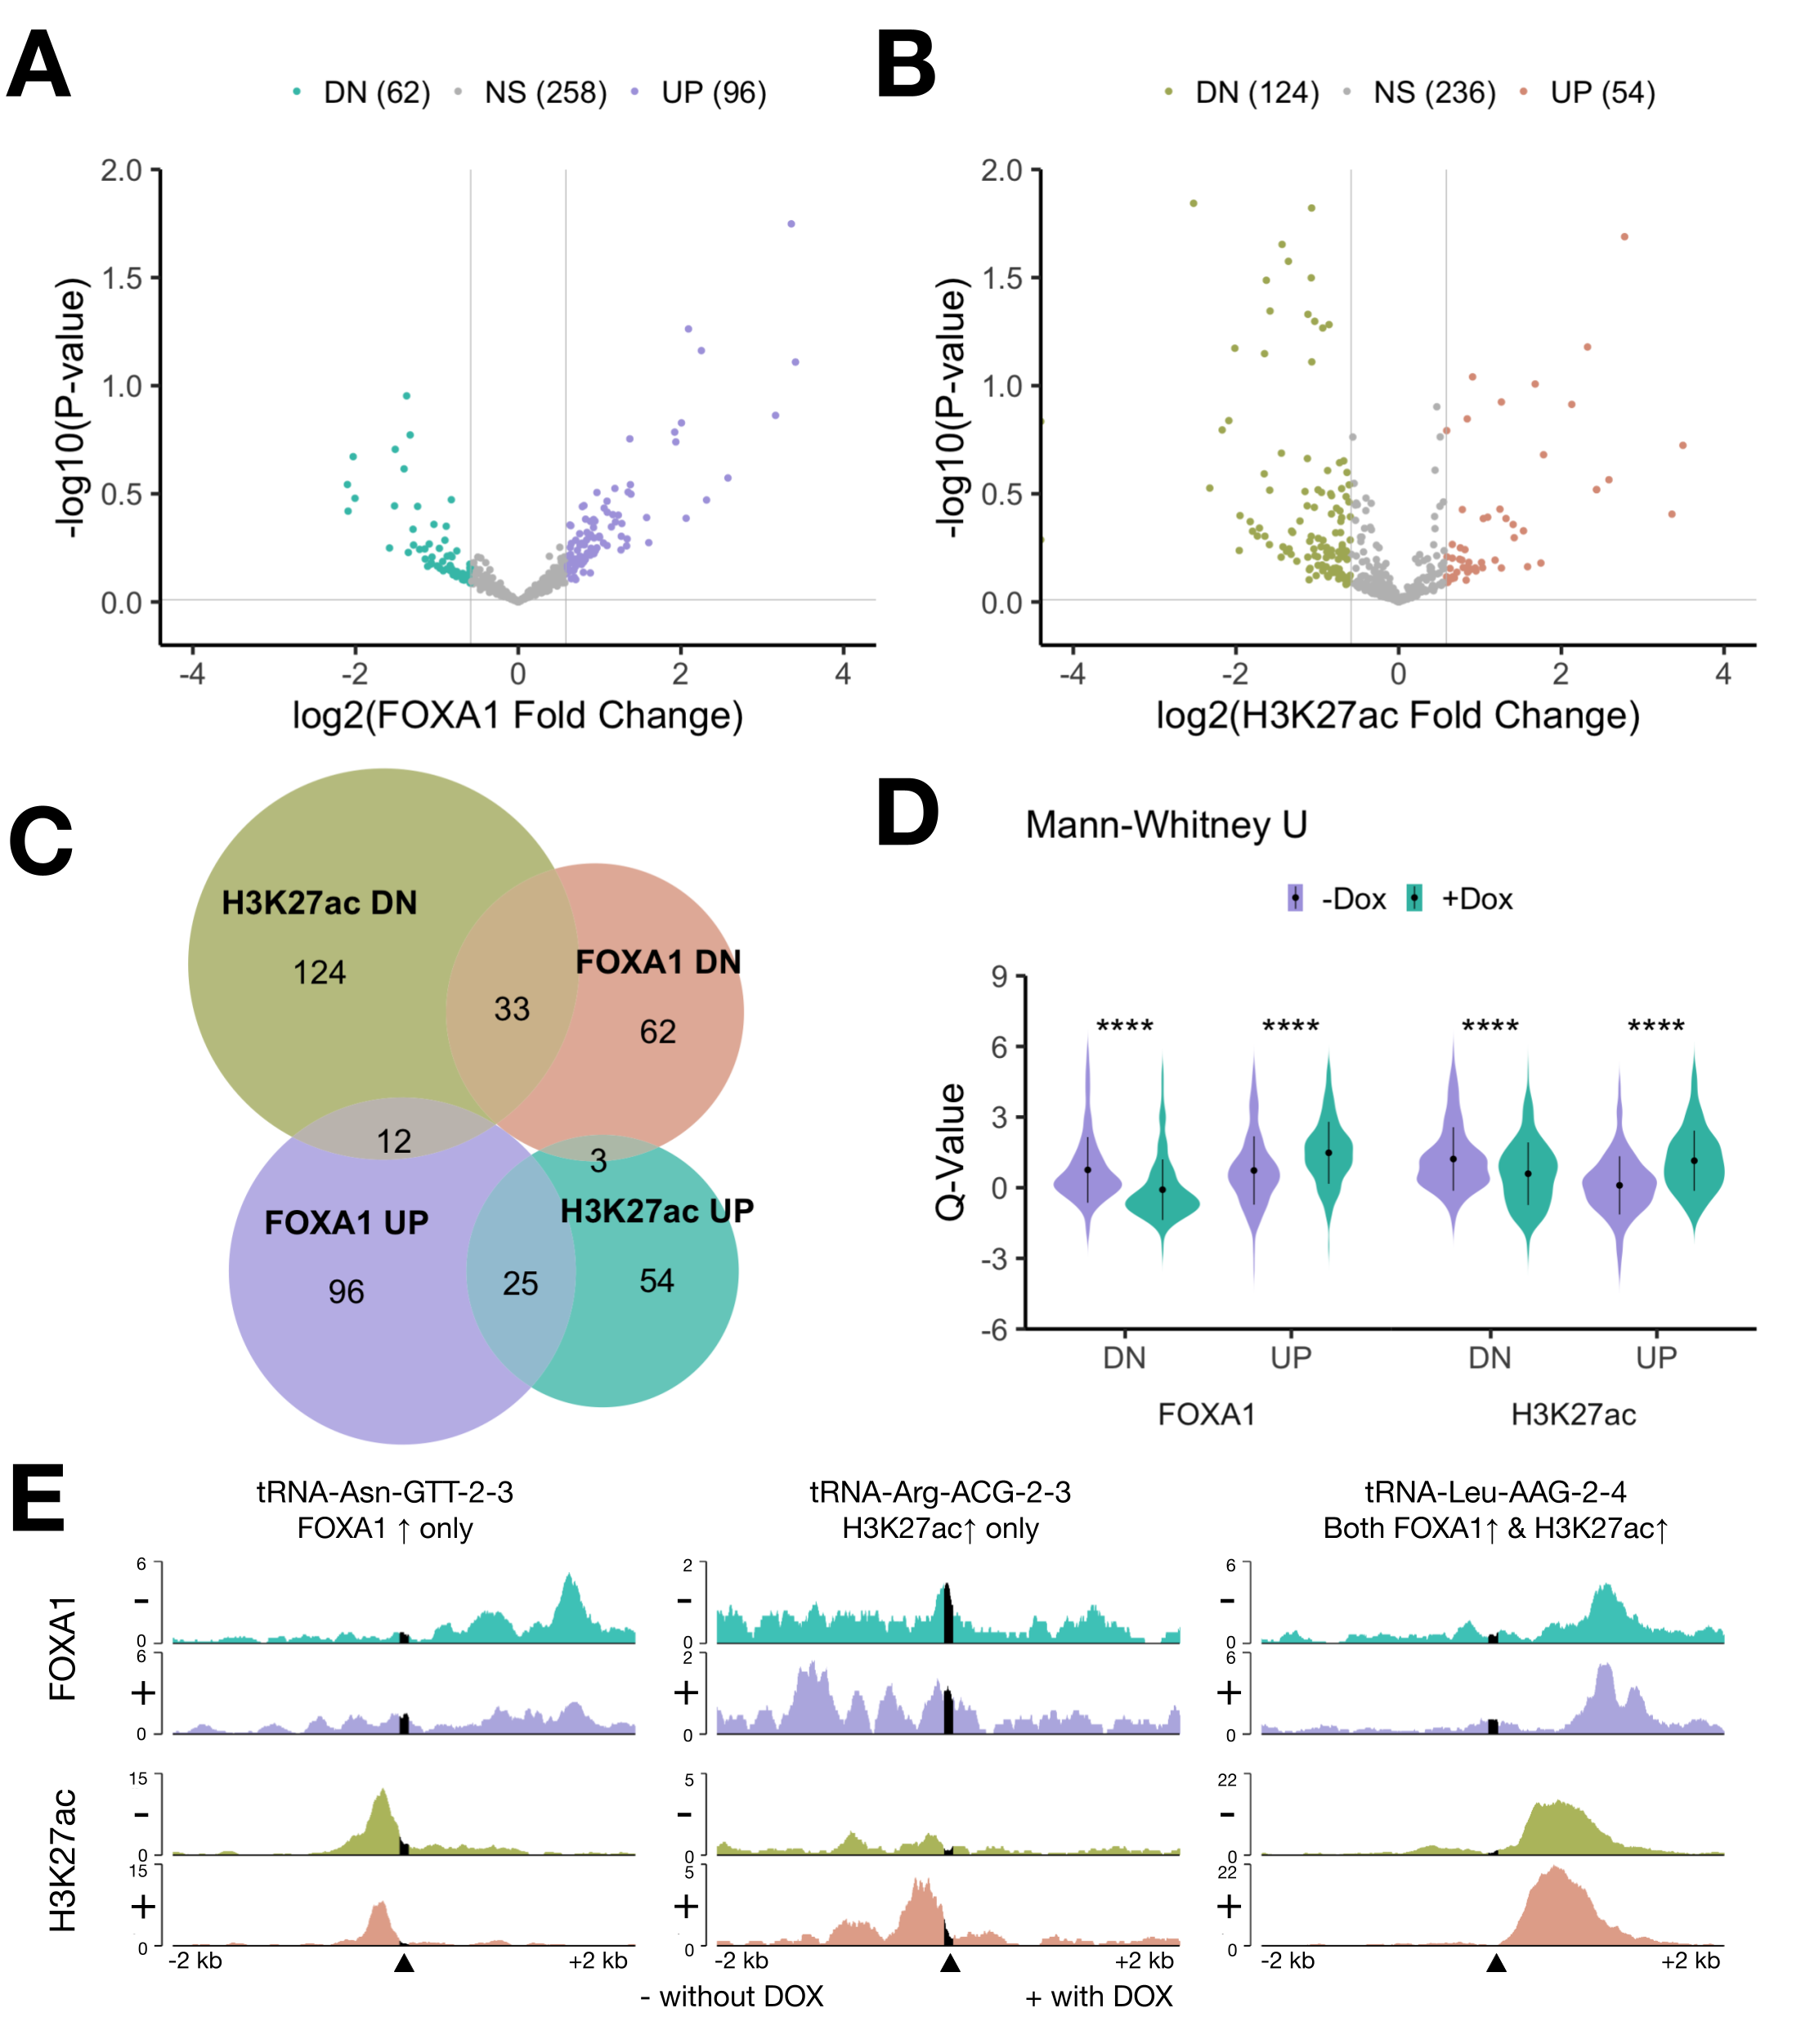
\includegraphics[width=1\linewidth]{../images/results-02} 

}

\caption{(B) Ratiometric heatmaps of the log2 ratio between the binding of FOXA1 or H3k27ac with endogenous FOXA1 expression vs. the binding of FOXA1 or H3k27ac with FOXA1 OE.}\label{fig:results-2}
\end{figure}

\hypertarget{figure-3}{%
\subsection{Figure 3}\label{figure-3}}

How many genes are `activated' by FOXA1?

What?

\begin{itemize}
\item
  tRNAs were classified as `active' if H3K27ac Q-values exceeded the median -DOX value (Q \textgreater{} 1.81).
\item
  How many genes are `active' in -DOX vs +DOX

  \begin{itemize}
  \item
    Number is similar
  \item
    Are +DOX genes the same genes?
    Compare -DOX and +DOX tRNA lists
  \item
    Parameter heatmap of GAIN/LOSS genes?
  \end{itemize}
\end{itemize}

Suggests?

\begin{figure}[H]

{\centering 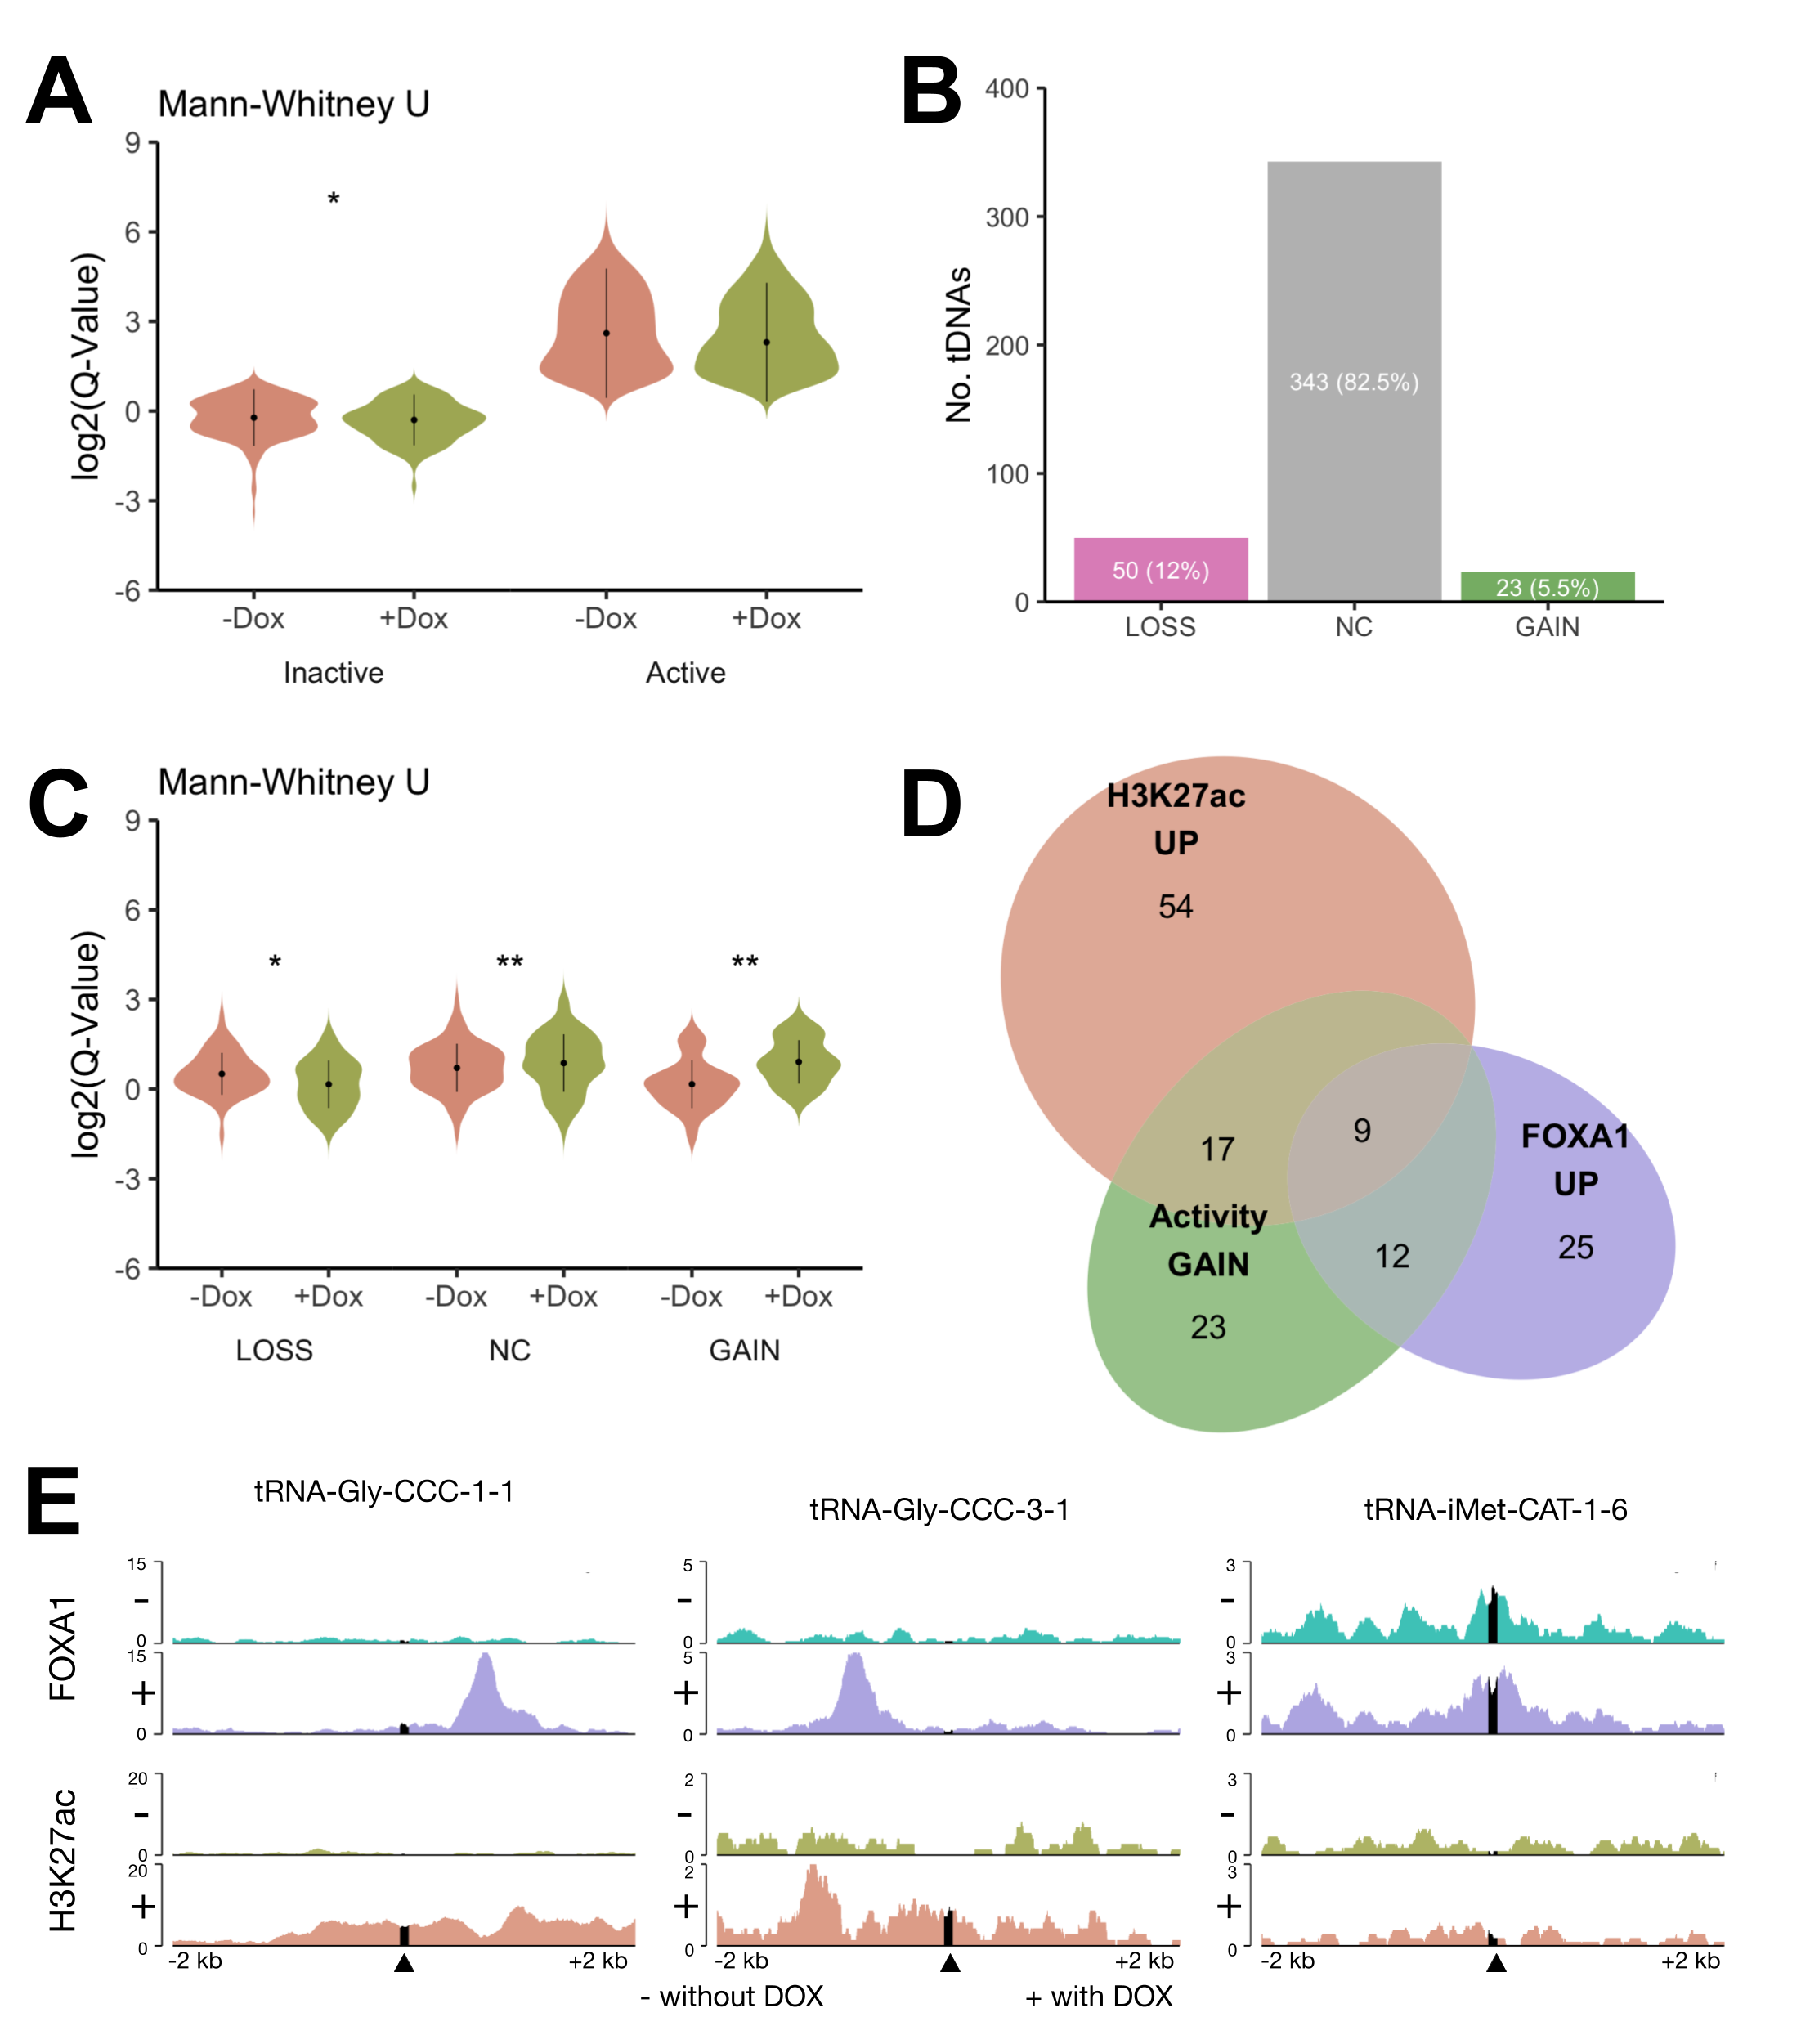
\includegraphics[width=1\linewidth]{../images/results-03} 

}

\caption{.}\label{fig:results-3}
\end{figure}

\hypertarget{figure}{%
\subsection{Figure ?}\label{figure}}

\begin{itemize}
\item
  Relative position (not very interesting)
\item
  Binding at isotopes?
  Certain AA more up than others?
\end{itemize}

\hypertarget{figure-4}{%
\subsection{Figure 4}\label{figure-4}}

\hypertarget{why-1}{%
\paragraph{Why?}\label{why-1}}

\hypertarget{what}{%
\subsubsection{What?}\label{what}}

MEME CentriMo to identify de novo motifs that are enriched at tRNAs which gain both FOXA1 and H3k27ac

\begin{itemize}
\item
  relative to other tRNAS (gain/lose, lose/lose, lose/gain)
\item
  FOXA1 not enriched
\item
  Look at ERE, AP-1, others?
\item
  Top 3 motifs (fisher E values) - IRF7, ERR3, NR4A1
\item
  A and B box motifs as a control?
  How?

  \begin{itemize}
  \item
    All downstream
  \item
    tRNAs where `matching sequences' all best matches = code for valine
  \item
    Branched amino acids associated with lower BC risk
  \end{itemize}
\end{itemize}

\hypertarget{suggests-1}{%
\paragraph{Suggests?}\label{suggests-1}}

\begin{figure}[H]

{\centering 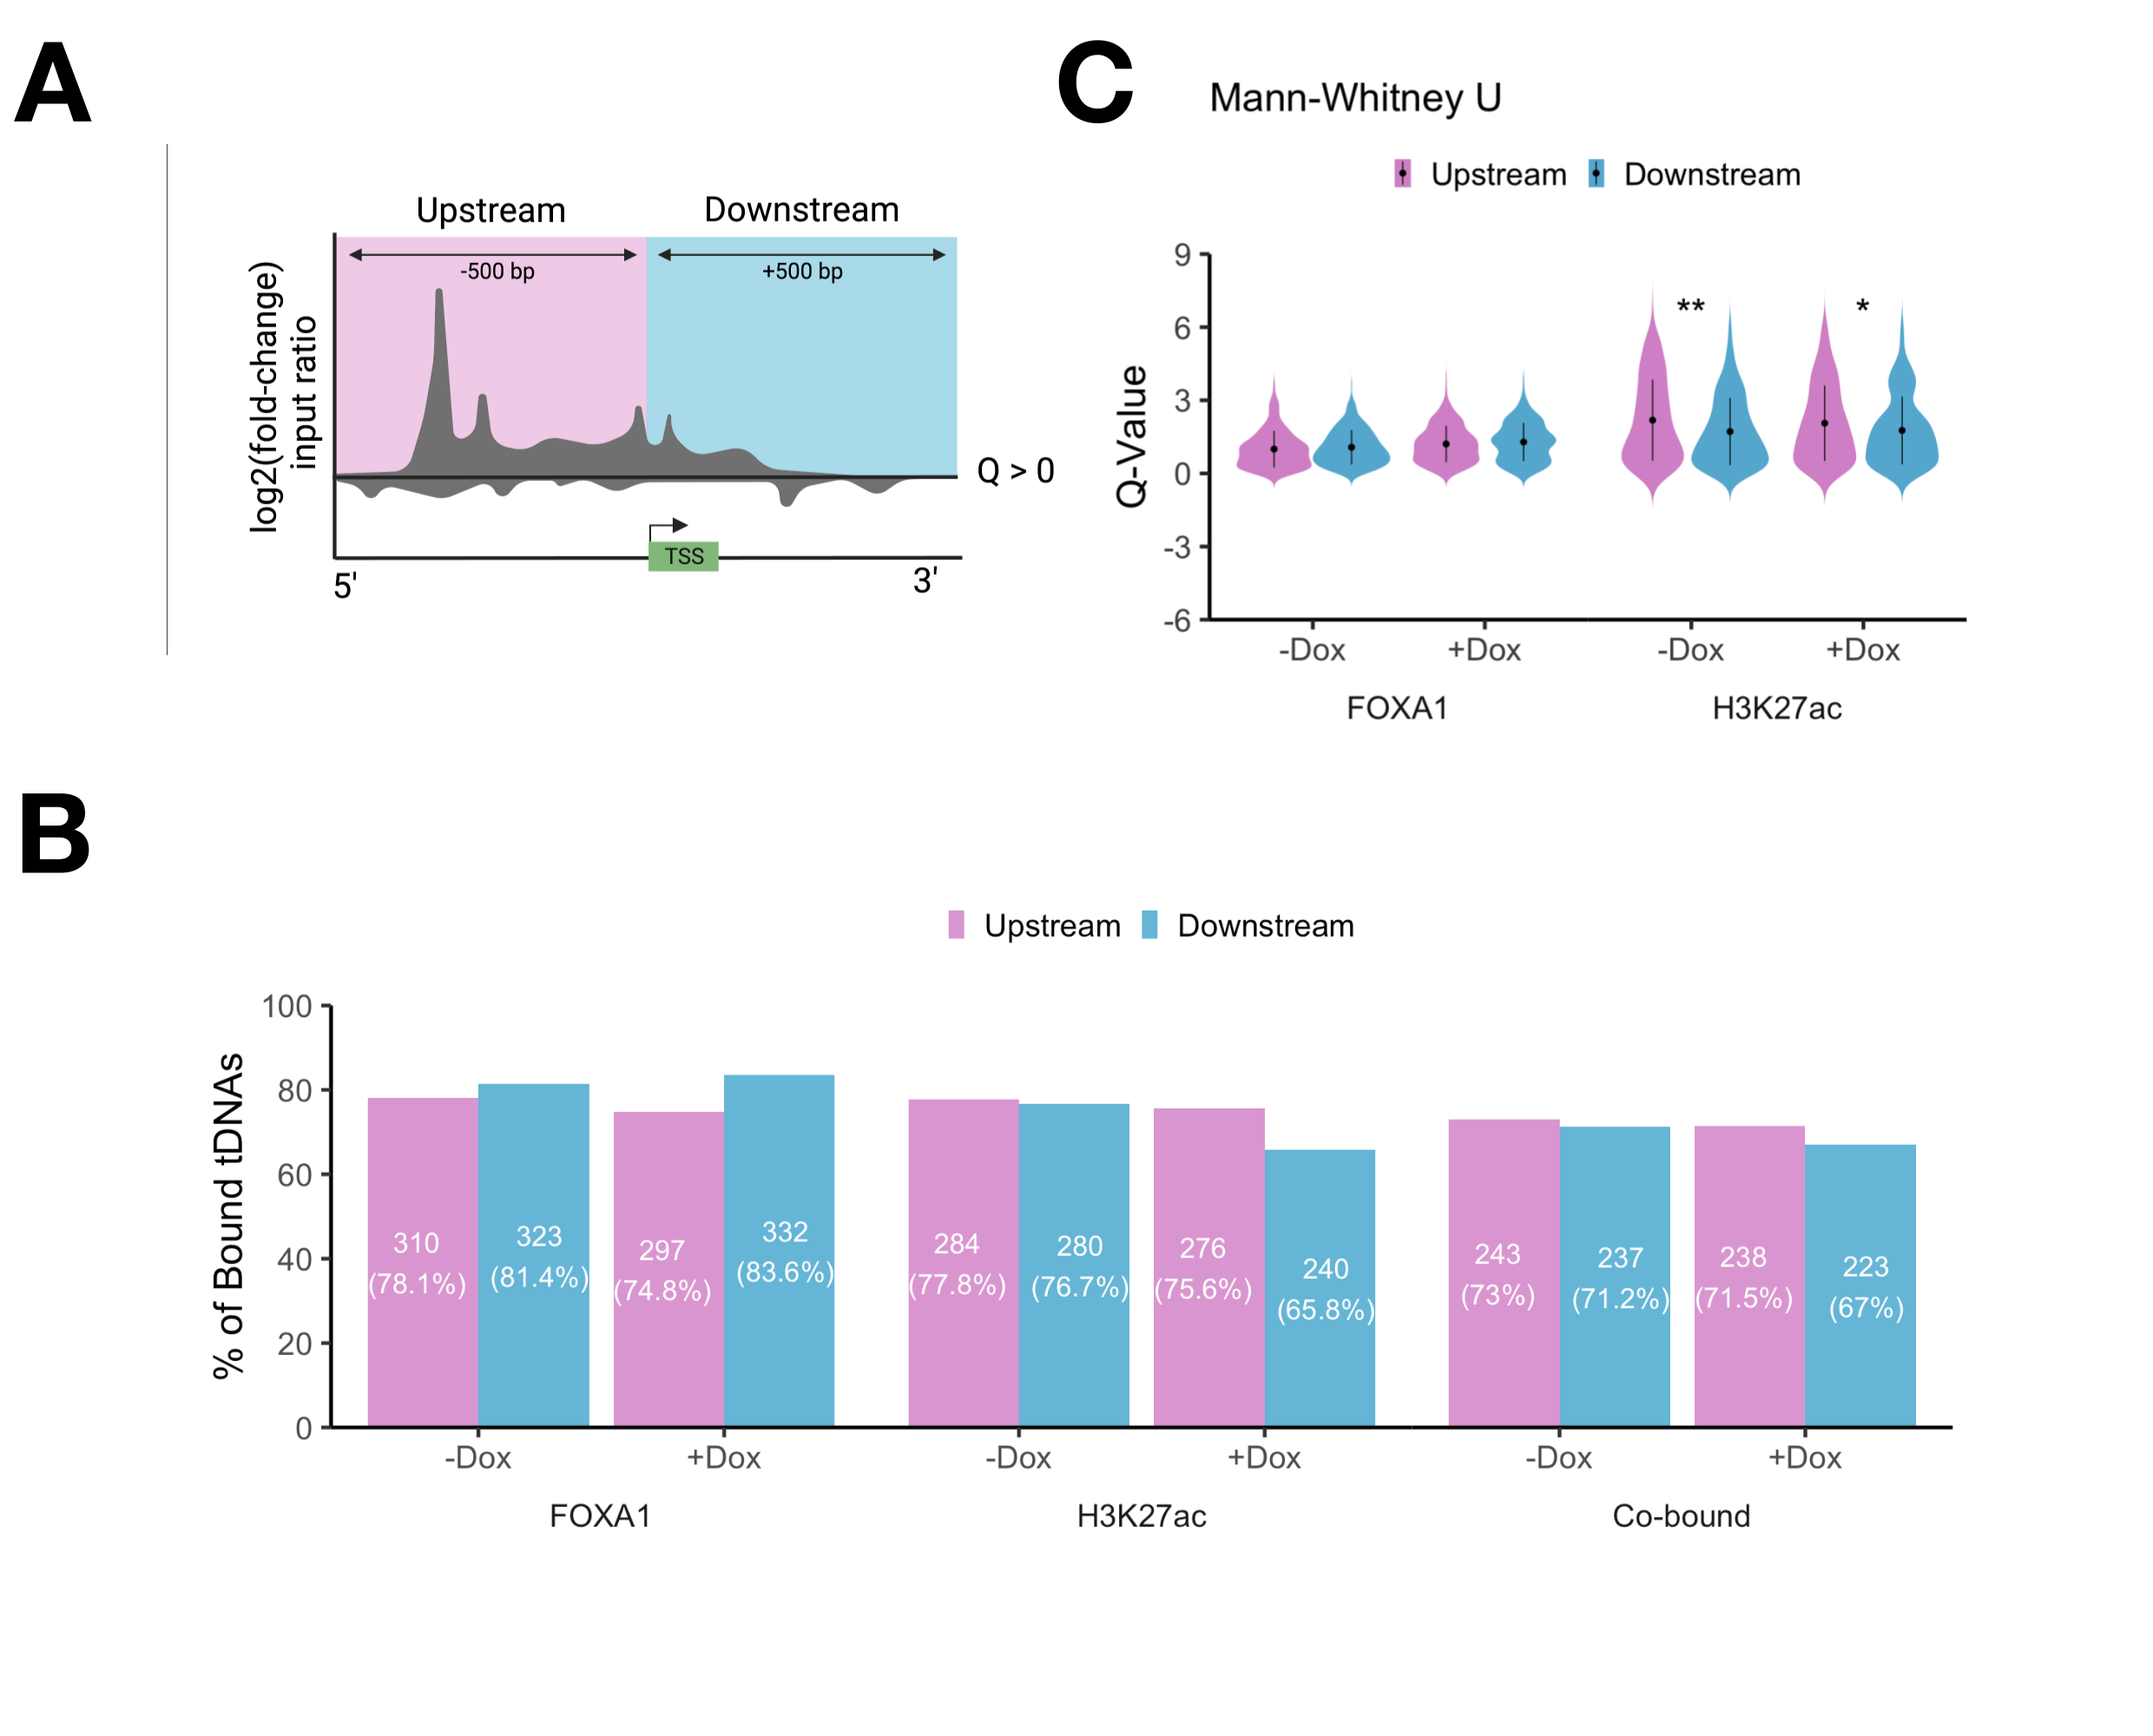
\includegraphics[width=1\linewidth]{../images/results-04} 

}

\end{figure}

\hypertarget{figure-5}{%
\subsection{Figure 5}\label{figure-5}}

\begin{itemize}
\tightlist
\item
  Localisation of FOXA1 at individual tRNA genes in MCF-7 cells
\end{itemize}

Why?

\begin{itemize}
\item
  tRNAs implicated in cancer
\item
  Are they upregulated?
\item
  Look at gain function/gain h3/fox
\item
  Motif ontology
\item
\end{itemize}

What?

Suggests?

\begin{longtable}[]{@{}ll@{}}
\caption{\label{tab:clusters}.}\tabularnewline
\toprule()
Group & Function \\
\midrule()
\endfirsthead
\toprule()
Group & Function \\
\midrule()
\endhead
ALOXE & Insulator Function\textsuperscript{{[}\protect\hyperlink{ref-raab2011}{11},\protect\hyperlink{ref-sizer2022}{12}{]}} \\
Ebersole & Insulator Function\textsuperscript{{[}\protect\hyperlink{ref-sizer2022}{12},\protect\hyperlink{ref-Ebersole2011}{13}{]}} \\
HES7 & \\
Per1 & \\
TMEM107 & Insulator Function\textsuperscript{{[}\protect\hyperlink{ref-raab2011}{11},\protect\hyperlink{ref-sizer2022}{12}{]}} \\
Arg-CCG & Implicated in Cancer Progression\textsuperscript{{[}\protect\hyperlink{ref-Goodarzi2016}{14}{]}} \\
Glu-TTC & Implicated in Cancer Progression\textsuperscript{{[}\protect\hyperlink{ref-Goodarzi2016}{14}{]}} \\
iMET & Proliferation of Breast Cancer \\
Met & iMet Control \\
SeC & Involved in REDOX\textsuperscript{{[}\protect\hyperlink{ref-Sangha2022}{15}{]}} \\
\bottomrule()
\end{longtable}

\begin{center}\rule{0.5\linewidth}{0.5pt}\end{center}

\hypertarget{discussion}{%
\section{Discussion}\label{discussion}}

\begin{itemize}
\item
  FOXA1 alone not efficient to increase activity

  \begin{itemize}
  \tightlist
  \item
    p300
  \end{itemize}
\item
  FOXA1 moves nucleosomes to make other TF accessible?
\item
  Loses fox = weak binding?
\item
  Dynamic vs stable marks
\item
  ATAC-seq
\end{itemize}

\hypertarget{conclusion}{%
\section{Conclusion}\label{conclusion}}

\begin{flushright}
997 Words
\end{flushright}

\begin{center}\rule{0.5\linewidth}{0.5pt}\end{center}

\hypertarget{references}{%
\section*{References}\label{references}}
\addcontentsline{toc}{section}{References}

\hypertarget{refs}{}
\begin{CSLReferences}{0}{0}
\leavevmode\vadjust pre{\hypertarget{ref-fu2019}{}}%
\CSLLeftMargin{1. }%
\CSLRightInline{Fu X, Pereira R, De Angelis C, Veeraraghavan J, Nanda S, Qin L, et al. FOXA1 upregulation promotes enhancer and transcriptional reprogramming in endocrine-resistant breast cancer. Proceedings of the National Academy of Sciences {[}Internet{]}. 2019 Dec 11;116(52):26823--34. Available from: \url{http://dx.doi.org/10.1073/pnas.1911584116}}

\leavevmode\vadjust pre{\hypertarget{ref-leinonen2010}{}}%
\CSLLeftMargin{2. }%
\CSLRightInline{Leinonen R, Sugawara H, Shumway M. The Sequence Read Archive. Nucleic Acids Research {[}Internet{]}. 2010 Nov 9;39(Database):D19--21. Available from: \url{http://dx.doi.org/10.1093/nar/gkq1019}}

\leavevmode\vadjust pre{\hypertarget{ref-thegala2022}{}}%
\CSLLeftMargin{3. }%
\CSLRightInline{Afgan E, Nekrutenko A, Grüning BA, Blankenberg D, Goecks J, Schatz MC, et al. The Galaxy platform for accessible, reproducible and collaborative biomedical analyses: 2022 update. Nucleic Acids Research {[}Internet{]}. 2022 Apr 21;50(W1):W345--51. Available from: \url{http://dx.doi.org/10.1093/nar/gkac247}}

\leavevmode\vadjust pre{\hypertarget{ref-langmead2012}{}}%
\CSLLeftMargin{4. }%
\CSLRightInline{Langmead B, Salzberg SL. Fast gapped-read alignment with Bowtie 2. Nature Methods {[}Internet{]}. 2012 Mar 4;9(4):357--9. Available from: \url{http://dx.doi.org/10.1038/nmeth.1923}}

\leavevmode\vadjust pre{\hypertarget{ref-Karolchik2004}{}}%
\CSLLeftMargin{5. }%
\CSLRightInline{Karolchik D. The UCSC Table Browser data retrieval tool. Nucleic Acids Research {[}Internet{]}. 2004 Jan 1;32(90001):493D--496. Available from: \url{http://dx.doi.org/10.1093/nar/gkh103}}

\leavevmode\vadjust pre{\hypertarget{ref-Chan2016}{}}%
\CSLLeftMargin{6. }%
\CSLRightInline{Chan PP, Lowe TM. GtRNAdb 2.0: an expanded database of transfer RNA genes identified in complete and draft genomes. Nucleic Acids Research {[}Internet{]}. 2015 Dec 15;44(D1):D184--9. Available from: \url{http://dx.doi.org/10.1093/nar/gkv1309}}

\leavevmode\vadjust pre{\hypertarget{ref-lerdrup2016}{}}%
\CSLLeftMargin{7. }%
\CSLRightInline{Lerdrup M, Johansen JV, Agrawal-Singh S, Hansen K. An interactive environment for agile analysis and visualization of ChIP-sequencing data. Nature Structural \& Molecular Biology {[}Internet{]}. 2016 Feb 29;23(4):349--57. Available from: \url{http://dx.doi.org/10.1038/nsmb.3180}}

\leavevmode\vadjust pre{\hypertarget{ref-r}{}}%
\CSLLeftMargin{8. }%
\CSLRightInline{R Core Team. R: A language and environment for statistical computing {[}Internet{]}. Vienna, Austria: R Foundation for Statistical Computing; 2023. Available from: \url{https://www.R-project.org/}}

\leavevmode\vadjust pre{\hypertarget{ref-rstudio}{}}%
\CSLLeftMargin{9. }%
\CSLRightInline{Posit Team. RStudio: Integrated development environment for r {[}Internet{]}. Boston, MA: Posit Software, PBC; 2023. Available from: \url{http://www.posit.co/}}

\leavevmode\vadjust pre{\hypertarget{ref-wickham2019}{}}%
\CSLLeftMargin{10. }%
\CSLRightInline{Wickham H, Averick M, Bryan J, Chang W, McGowan L, François R, et al. Welcome to the tidyverse. Journal of Open Source Software {[}Internet{]}. 2019 Nov 21;4(43):1686. Available from: \url{http://dx.doi.org/10.21105/joss.01686}}

\leavevmode\vadjust pre{\hypertarget{ref-raab2011}{}}%
\CSLLeftMargin{11. }%
\CSLRightInline{Raab JR, Chiu J, Zhu J, Katzman S, Kurukuti S, Wade PA, et al. Human tRNA genes function as chromatin insulators. The EMBO Journal {[}Internet{]}. 2011 Nov 15;31(2):330--50. Available from: \url{http://dx.doi.org/10.1038/emboj.2011.406}}

\leavevmode\vadjust pre{\hypertarget{ref-sizer2022}{}}%
\CSLLeftMargin{12. }%
\CSLRightInline{Sizer RE, Chahid N, Butterfield SP, Donze D, Bryant NJ, White RJ. TFIIIC-based chromatin insulators through eukaryotic evolution. Gene {[}Internet{]}. 2022 Aug;835:146533. Available from: \url{http://dx.doi.org/10.1016/j.gene.2022.146533}}

\leavevmode\vadjust pre{\hypertarget{ref-Ebersole2011}{}}%
\CSLLeftMargin{13. }%
\CSLRightInline{Ebersole T, Kim J-H, Samoshkin A, Kouprina N, Pavlicek A, White RJ, et al. tRNA genes protect a reporter gene from epigenetic silencing in mouse cells. Cell Cycle {[}Internet{]}. 2011 Aug 15;10(16):2779--91. Available from: \url{http://dx.doi.org/10.4161/cc.10.16.17092}}

\leavevmode\vadjust pre{\hypertarget{ref-Goodarzi2016}{}}%
\CSLLeftMargin{14. }%
\CSLRightInline{Goodarzi H, Nguyen HCB, Zhang S, Dill BD, Molina H, Tavazoie SF. Modulated Expression of Specific tRNAs Drives Gene Expression and Cancer Progression. Cell {[}Internet{]}. 2016 Jun;165(6):1416--27. Available from: \url{http://dx.doi.org/10.1016/j.cell.2016.05.046}}

\leavevmode\vadjust pre{\hypertarget{ref-Sangha2022}{}}%
\CSLLeftMargin{15. }%
\CSLRightInline{Sangha AK, Kantidakis T. The Aminoacyl-tRNA Synthetase and tRNA Expression Levels Are Deregulated in Cancer and Correlate Independently with Patient Survival. Current Issues in Molecular Biology {[}Internet{]}. 2022 Jul 2;44(7):3001--19. Available from: \url{http://dx.doi.org/10.3390/cimb44070207}}

\end{CSLReferences}

\end{document}
